\documentclass[11pt]{article}
\usepackage[T1]{fontenc}
\usepackage{lmodern}
\usepackage{tikz}
\usepackage{pgfplots}
\pgfplotsset{compat=1.18}
\usepackage{circuitikz}
\usetikzlibrary{arrows.meta,positioning,calc}
\usepackage{caption}
\begin{document}

\section{Pictures in a document}

A document with many drawings is where background passes get slow: every TikZ picture is
drawn again on every pass, whether or not anything near it changed. The session keeps the
pictures of an earlier pass and reuses them, so a pass costs the text, not the drawings.

\begin{center}
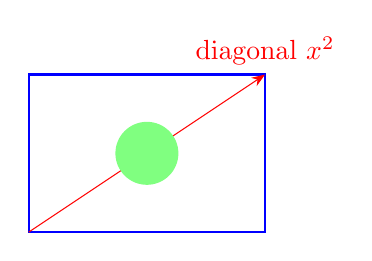
\begin{tikzpicture}
  \draw[thick,blue] (0,0) rectangle (3,2);
  \draw[red,-{Stealth}] (0,0) -- (3,2) node[above] {diagonal $x^2$};
  \fill[green!50] (1.5,1) circle (0.4);
\end{tikzpicture}
\end{center}

An inline picture \begin{tikzpicture}[baseline]\draw (0,0) -- (1,0.5) circle (2pt);\end{tikzpicture}
sits inside a sentence that goes on for a while and wraps onto a second line of the page, and a short
\tikz\draw[fill=orange] (0,0) circle (3pt); dot as well.

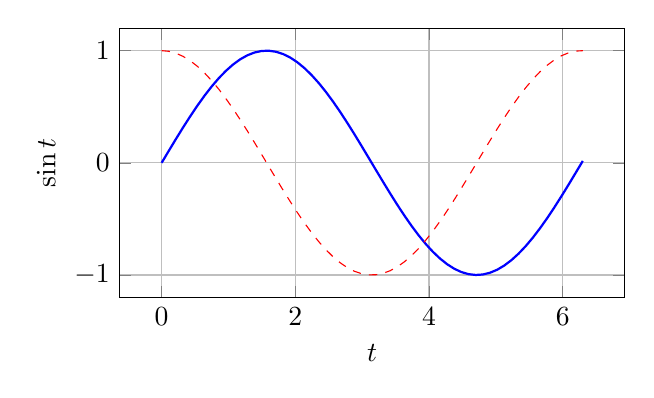
\begin{tikzpicture}
  \begin{axis}[width=8cm,height=5cm,xlabel=$t$,ylabel=$\sin t$,grid=major]
    \addplot[domain=0:6.3,samples=60,blue,thick] {sin(deg(x))};
    \addplot[domain=0:6.3,samples=60,red,dashed] {cos(deg(x))};
  \end{axis}
\end{tikzpicture}

\def\R{1.2}
\begin{center}
\begin{tikzpicture}
  \draw (0,0) circle (\R);
  \foreach \a in {0,45,...,315} { \draw (0,0) -- (\a:\R); }
  \node at (0,-\R-0.4) {spokes};
\end{tikzpicture}
\end{center}

Text after the circle. The circle's radius comes from a macro defined just before it: the
picture's hash includes that definition, so changing the radius redraws the picture.

\begin{center}
  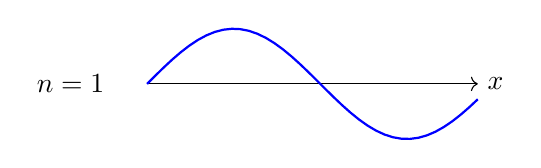
\begin{tikzpicture}[scale=1.4, baseline={($(current bounding box.center)$)}]
    \draw[->] (0,0) -- (3,0) node[right] {$x$};
    \draw[thick,blue] plot[domain=0:3,samples=40] (\x,{0.5*sin(2*\x r)});
    \node at (-0.3,0) [anchor=east] {$n=1$};
  \end{tikzpicture}
  \hfill
  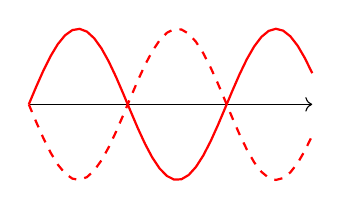
\begin{tikzpicture}[scale=1.2, baseline={($(current bounding box.center)$)}]
    \draw[->] (0,0) -- (3,0);
    \draw[thick,red] plot[domain=0:3,samples=40] (\x,{0.8*sin(3*\x r)});
    \draw[thick,red,dashed] plot[domain=0:3,samples=40] (\x,{-0.8*sin(3*\x r)});
  \end{tikzpicture}
  \\
  $^*$: two pictures on one line, each with its baseline at its centre.
\end{center}

\begin{itemize}
  \item
  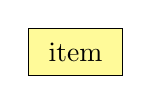
\begin{tikzpicture}[baseline=(current bounding box.center)]
    \draw[fill=yellow!40] (0,0) rectangle (1.2,0.6) node[midway] {item};
  \end{tikzpicture}
  a picture that starts a list item: the label is placed by the paragraph, not by the
  picture, and must not end up inside the cached image.
  \item A plain item after it.
\end{itemize}

\subsection{A circuit}

\begin{figure}[htbp]
\centering
\begin{circuitikz}[american]
  \draw (0,0) to[battery1, l=$V$] (0,3)
        to[R, l=$R_1$] (3,3)
        to[R, l=$R_2$] (3,0) -- (0,0);
  \draw (3,3) to[short, -o] (4.5,3);
  \draw (3,0) to[short, -o] (4.5,0);
\end{circuitikz}
\caption{A voltage divider.}
\label{fig:divider}
\end{figure}

Figure~\ref{fig:divider} is a float: the picture inside it is cached like any other, the
float itself is placed by the pass as usual.


\begin{tikzpicture}
  \node[draw] (a) {Section \ref{sec:second}};
  \node[draw,right=of a] (b) {page \pageref{sec:second}};
  \draw[->] (a) -- (b);
\end{tikzpicture}

The picture above refers to a label, so it is never cached: its text depends on the aux file,
which changes between passes.

\newpage
\section{Second page}
\label{sec:second}

Pictures on a later page come from that page of the earlier pass's PDF.

\begin{center}
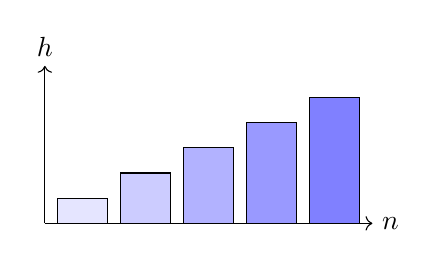
\begin{tikzpicture}[scale=0.8]
  \foreach \i in {1,...,5} {
    \draw[fill=blue!\i0] (\i,0) rectangle ++(0.8,{\i*0.4});
  }
  \draw[->] (0.8,0) -- (6,0) node[right] {$n$};
  \draw[->] (0.8,0) -- (0.8,2.5) node[above] {$h$};
\end{tikzpicture}
\end{center}

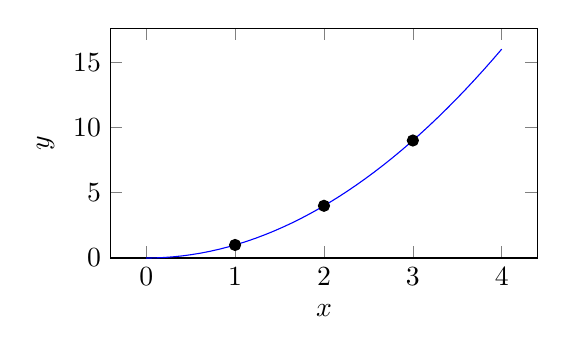
\begin{tikzpicture}
  \begin{axis}[width=7cm,height=4.5cm,xlabel=$x$,ylabel=$y$,ymin=0]
    \addplot[domain=0:4,samples=40,blue] {x^2};
    \addplot[only marks,mark=*] coordinates {(1,1) (2,4) (3,9)};
  \end{axis}
\end{tikzpicture}

A closing paragraph with ordinary text, which the fast path handles while the pictures stay
as they were drawn.
\end{document}
